%%%%%%%%%%%%%%%%%%%%%%%%%%%%%%%%%%%%%%%%%%%%%%%%%%%%%%%%%%%%%%%%%%%%
%% I, the copyright holder of this work, release this work into the
%% public domain. This applies worldwide. In some countries this may
%% not be legally possible; if so: I grant anyone the right to use
%% this work for any purpose, without any conditions, unless such
%% conditions are required by law.
%%%%%%%%%%%%%%%%%%%%%%%%%%%%%%%%%%%%%%%%%%%%%%%%%%%%%%%%%%%%%%%%%%%%

\documentclass[
  digital,     %% The `digital` option enables the default options for the
               %% digital version of a document. Replace with `printed`
               %% to enable the default options for the printed version
               %% of a document.
%%  color,       %% Uncomment these lines (by removing the %% at the
%%               %% beginning) to use color in the printed version of your
%%               %% document
  oneside,     %% The `oneside` option enables one-sided typesetting,
               %% which is preferred if you are only going to submit a
               %% digital version of your thesis. Replace with `twoside`
               %% for double-sided typesetting if you are planning to
               %% also print your thesis. For double-sided typesetting,
               %% use at least 120 g/m² paper to prevent show-through.
  nosansbold,  %% The `nosansbold` option prevents the use of the
               %% sans-serif type face for bold text. Replace with
               %% `sansbold` to use sans-serif type face for bold text.
  nocolorbold, %% The `nocolorbold` option disables the usage of the
               %% blue color for bold text, instead using black. Replace
               %% with `colorbold` to use blue for bold text.
  lof,         %% The `lof` option prints the List of Figures. Replace
               %% with `nolof` to hide the List of Figures.
  lot,         %% The `lot` option prints the List of Tables. Replace
               %% with `nolot` to hide the List of Tables.
]{fithesis4}
%% The following section sets up the locales used in the thesis.
\usepackage[resetfonts]{cmap} %% We need to load the T2A font encoding
\usepackage[T1,T2A]{fontenc}  %% to use the Cyrillic fonts with Russian texts.
\usepackage[
  main=english, %% By using `czech` or `slovak` as the main locale
                %% instead of `english`, you can typeset the thesis
                %% in either Czech or Slovak, respectively.
  english, german, czech, slovak %% The additional keys allow
]{babel}        %% foreign texts to be typeset as follows:
%%
%%   \begin{otherlanguage}{german}  ... \end{otherlanguage}
%%   \begin{otherlanguage}{czech}   ... \end{otherlanguage}
%%   \begin{otherlanguage}{slovak}  ... \end{otherlanguage}
%%
%%
%% The following section sets up the metadata of the thesis.
\thesissetup{
    date        = \the\year/\the\month/\the\day,
    university  = mu,
    faculty     = fi,
    type        = bc,
    department  ={Department of Computer Systems and Communications},
    author      = Jindřich Halabala,
    gender      = m,
    advisor     = {RNDr. Ondřej Krajíček},
    title       = {Experimenting with web-page structural analysis using Deep Reinforcement Learning},
    TeXtitle    = {Experimenting with web-page structural analysis using Deep Reinforcement Learning},
    keywords    = {TODO, keyword2, ...},
    TeXkeywords = {TODO, keyword2, \ldots},
    abstract    = {%
      This is the abstract of my thesis, which can

      span multiple paragraphs.
    },
    thanks      = {%
      These are the acknowledgements for my thesis, which can

      span multiple paragraphs.
    },
    bib         = example.bib,
    %% Remove the following line to use the JVS 2018 faculty logo.
    facultyLogo = fithesis-fi,
}
\usepackage{makeidx}      %% The `makeidx` package contains
\makeindex                %% helper commands for index typesetting.
%% These additional packages are used within the document:
\usepackage{paralist} %% Compact list environments
\usepackage{amsmath}  %% Mathematics
\usepackage{amsthm}
\usepackage{amsfonts}
\usepackage{url}      %% Hyperlinks
\usepackage{markdown} %% Lightweight markup
\usepackage{listings} %% Source code highlighting
\usepackage{svg}      %% SVG figures
\lstset{
  basicstyle      = \ttfamily,
  identifierstyle = \color{black},
  keywordstyle    = \color{blue},
  keywordstyle    = {[2]\color{cyan}},
  keywordstyle    = {[3]\color{olive}},
  stringstyle     = \color{teal},
  commentstyle    = \itshape\color{magenta},
  breaklines      = true,
}
\usepackage{floatrow} %% Putting captions above tables
\floatsetup[table]{capposition=top}
\usepackage[babel]{csquotes} %% Context-sensitive quotation marks
\begin{document}
%% The \chapter* command can be used to produce unnumbered chapters:
\chapter*{Introduction}
%% Unlike \chapter, \chapter* does not update the headings and does not
%% enter the chapter to the table of contents. I we want correct
%% headings and a table of contents entry, we must add them manually:
\markright{\textsc{Introduction}}
\addcontentsline{toc}{chapter}{Introduction}

TODO

\chapter{User interface element detection}

Y Soft AIVA\footnote{\url{https://www.ysoft.com/aiva}} is a software solution for automated end-to-end testing of web applications. Unlike most competitors, AIVA does not interact with the web page's Document Object Model (DOM). Instead, it relies entirely on visual information. This approach closely resembles how a real user interacts with the application (black-box testing) and enhances robustness in specific scenarios, such as when XPaths change due to newly added components. However, it also presents many challenges since all the information must be extracted from an image instead of a markup language.

A crucial aspect of data extraction is identifying the location, size, and hierarchical relationships of all key interactable elements on a web page (e.g., buttons, icons, text fields). If this step is done correctly, it allows AIVA to reconstruct the DOM and localize correct elements during test execution.

This process can be approached using both detection and segmentation, as most objects on a webpage are rectangular. However, due to the hierarchical nature of the DOM, detection is a more intuitive choice, as a single pixel can belong to multiple overlapping elements. That said, the detected information can be converted into a segmentation map if needed. This correspondence is visible in Figure~\ref{fig:example-result}.

\begin{figure}
    \centering
    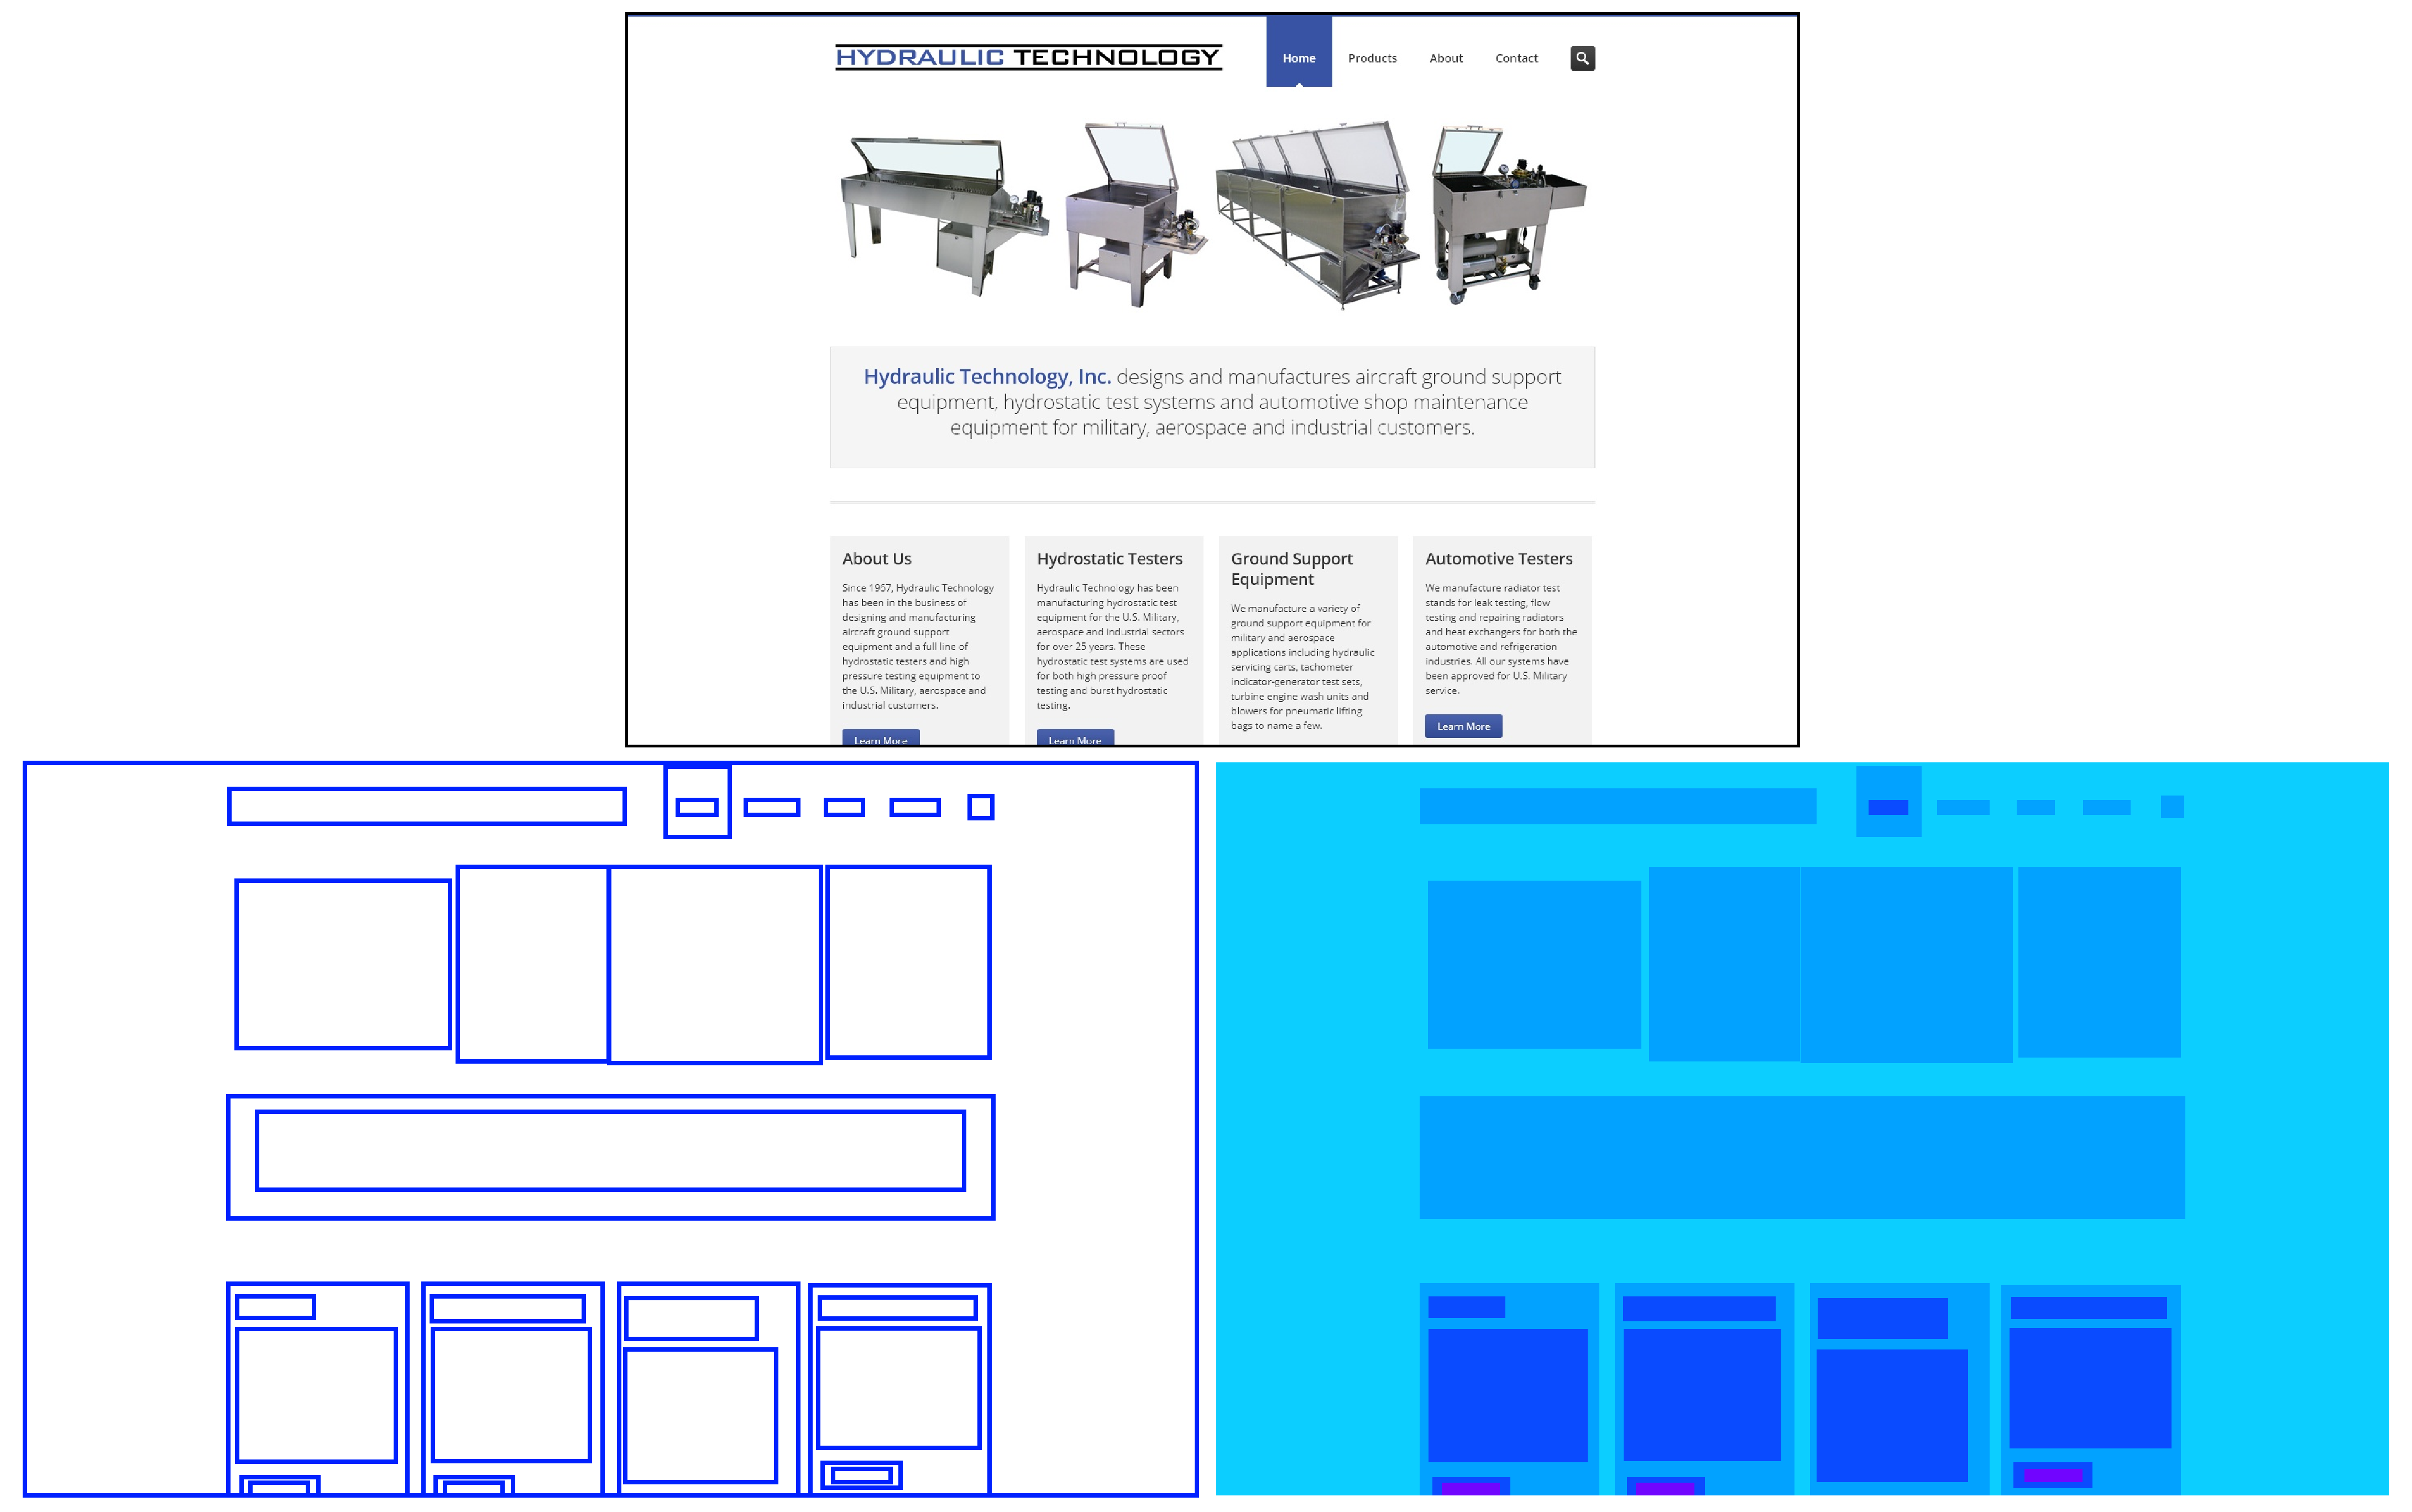
\includegraphics[width=0.7\linewidth]{diagrams/result_example.pdf}
    \caption{An example of a processed web page. The top image is the original screenshot, the middle image shows bounding boxes of detection, and the bottom image shows the same but as a segmentation map. The original screenshot comes from~\cite{aydos2020}.}
    \label{fig:example-result}
\end{figure}

Graphical user interface (GUI) object detection is usually done using traditional computer vision (CV), deep learning-based object detection models such as R-CNNs or YOLO, or by a combination of both (for example, using a deep learning (DL) model for text and image detection and CV for the rest)~\cite{ODforGUI_CV_DL_or_both}. This chapter looks at both approaches, some existing solutions based upon them, and the challenges they present. Finally, a third approach that could solve these problems is proposed based on deep reinforcement learning.

\section{Traditional computer vision-based solutions}

Traditional computer vision is used in this thesis to describe algorithms for digital image processing that do not utilize machine learning, instead operating on a pixel-by-pixel basis. Tradition CV is challenging to use for object detection in photographs due to noise and unclear edges but is well-suited for processing user interfaces. Screenshots usually do not contain any noise (at most, some compression artifacts might be present), and edges are clearly defined.

The most common technique is using an edge detection method (e.g., Canny or Sobel edge detection) followed by some extra processing to make the edges cleaner (e.g., morphological operations, filtering of small edges), and finally, detecting contours in the binary image. This process is then commonly combined with results from an optical character recognition (OCR) model and further processed to merge similar elements and filter out small elements that are likely just noise. We can find this exact process in algorithms such as REMAUI~\cite{remaui} (a program for reverse engineering of mobile application GUIs), UISeg~\cite{uiseg} (user interface segmentation algorithm), and also in the current implementation of AIVA's element detection procedure.

Template matching is another approach for localization, but it lacks flexibility. It works reliably for highly standardized elements (e.g., checkboxes or buttons in desktop applications with a fixed GUI style). However, it is ineffective for mobile or web applications where GUI components vary widely in design~\cite{ODforGUI_CV_DL_or_both}.

Even today, with the rapid progress in deep learning, traditional CV still offers some benefits compared to it. It can be much more efficient and straightforward to understand, making it much easier to modify and debug. We can observe the results of each step of the algorithm, see what went wrong, and adjust parameters and thresholds accordingly. These sorts of modifications are difficult to achieve with DL. Another significant benefit is the reduced dependency on large training datasets, which often require a lot of manual labor to create. This reliance also means DL-based models can become obsolete if the design trends of GUIs change~\cite{DLvsTCV}.

\section{Deep learning-based solutions}
In the last ten years, state-of-the-art object detection algorithms have been almost solely based on deep neural networks with convolutional layers. Region-based Convolutional Neural Networks (R-CNNs) and You Only Look Once (YOLO) are the two most prominent model families. Generally, R-CNNs offer higher accuracy, while YOLO provides better speed, though performance varies by model and use case~\cite{ObjectDetectionHistorySurvey}.

An example of a deep learning-based GUI element detection algorithm is OmniParser\footnote{\url{https://microsoft.github.io/OmniParser/}}~, a fine-tuned YOLOv8 model for parsing and labeling GUIs. It was created to improve the performance of large multi-modal agents like GPT-4V~\cite{OmniParser}. In~\cite{GUI_YOLO_comparison}, Daneshvar et al. tried training different YOLO architectures for GUI element detection with good results. When AIVA was primarily used to test physical devices with touch screens, it used a model based on the Single Shot Detection architecture for element detection~\cite{Horak2020thesis}.

A key advantage of DL-based solutions is their ability to learn complex patterns from data without explicit programming or manual tuning for a specific domain. However, as stated in the previous section, this reliance on a dataset is also one of the main drawbacks. Both training and inference are also more hardware demanding than most traditional CV algorithms~\cite{DLvsTCV}.

\section{Object detection with reinforcement learning}

The previous two sections highlight two significant challenges. Traditional CV is insufficient for more complex images, and DL requires a large, high-quality dataset. A combination of both could, in theory, eliminate or at least mitigate these drawbacks. It should be possible to create a function that evaluates the quality of a bounding box prediction based on traditional CV techniques. This function could then serve as a supervisory signal for training a deep learning model, removing the need for a dataset with manually labeled ground truth bounding boxes. Instead, only images of web applications would be required, which are significantly easier to obtain.

Supervised learning models are not applicable if we only have a numerical score for predictions rather than ground truth labels. Instead, we can use a reinforcement learning model that learns from evaluative feedback (more details on RL in Chapter~\ref{ch:dlr}).

To my best knowledge, no author investigated multi-object detection using reinforcement learning. However, there have been papers on using it to detect a single object in photographs~\cite{dlr_object_detection, iterative_od_with_rl, hierarchical_od_with_drl} and for region proposal in multi-object detection~\cite{drl_rpn}. They all use ground-truth labels for learning since creating a CV-based reward function for photographs would be very difficult. However, for GUIs, it should be feasible. 

\chapter{Deep reinforcement learning}
\label{ch:dlr}

To understand the terminology used and decisions made in the following chapters, it is important to first have a basic understanding of the theory behind reinforcement learning and machine learning in general. This chapter should provide enough information to understand the rest of this thesis. Please note that it is only a brief introduction to the topic; only the most important algorithms and definitions are provided. It is definitely not exhaustive.

Unless stated otherwise, the notation and information used in this chapter are from the book \textit{Grokking Deep Reinforcement Learning} by Miguel Morales~\cite{GDRL}.

\section{Machine learning}
Machine learning (ML) is the study of algorithms that allow computers to learn from data without explicit programming. It is often split into three main categories: supervised learning, unsupervised learning, and reinforcement learning\footnote{Other categories, such as semi-supervised or self-supervised learning, are also sometimes stated, but they are usually just modifications of the three main categories.}~\cite{IB031}.

In supervised learning (SL), the goal is to learn to make predictions when the correct answers are available during training. This is ideal for classification or regression, where the correct labels are known (be it from human labeling, automated data collection, or some other method)~\cite{IB031}.

In unsupervised learning (UL), no correct labels are known, so it is more about finding patterns in the provided data. This can be used to, for example, separate the data into groups (clustering) or to generate new data similar to the provided examples (autoencoders, generative adversarial networks) [ZDROJ???? Asi IB031 pro definici a PV021 pro příklady].

Similar to SL, reinforcement learning involves learning a mapping from inputs to outputs. However, unlike in SL, where the correct labels are provided for training purposes, RL relies only on the feedback from a reward function. This function evaluates the agent's actions based on their outcomes, providing scalar feedback that indicates the quality of those actions. The agent's goal is to learn to make decisions that maximize this reward through trial and error. This makes RL ideal for decision-making, especially in environments where we do not have access to the optimal strategy.

\section{Reinforcement learning}
Reinforcement learning problems are composed of two entities that interact -- the agent and the environment. The agent is the algorithm taught to make decisions. The environment is everything else -- if the goal is to drive a car, then the environment contains all the other cars, their movement, the roads, pedestrians, and also the car the agent is controlling. The agent tries to interact with the environment in such a way that maximizes the reward.

The typical interaction between agent and environment in RL follows a cycle. In the beginning, the environment is in some initial state. The agent observes the state (note that the observation can contain only a part of the state) and, based on this observation, decides to perform an action. The environment reacts to this action, changing its inner state. The agent observes this new state and also receives a reward based on the action. The agent can then learn based on this feedback and change its behavior. It then again chooses an action, and the cycle repeats as shown in figure \ref{fig:rl-cycle}.

\begin{figure}
    \centering
    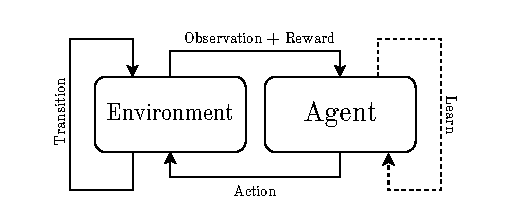
\includegraphics[width=1\linewidth]{diagrams/rl_cycle.pdf}
    \caption{The reinforcement learning cycle}
    \label{fig:rl-cycle}
\end{figure}

One iteration of this cycle is called a time step, and it creates an experience -- a tuple of the original state $s$, the action taken $a$, the reward given $r$, and the new state $s'$. Depending on the task, this cycle can repeat forever or end once the environment reaches some terminal state. For example, in a game of chess, the end is defined as winning, losing, or a draw. We call such tasks episodic, and all the experiences collected from the initial to the terminal states form an episode. If there is no well-defined end, we call the task continuous.

Reinforcement learning is challenging due to the feedback being sequential, evaluative, and sampled.

The sequentiality comes from most of the tasks being multiple steps long, and thus, the consequences of an action might not be apparent immediately. When an episode ends with a very negative result, it can be hard to figure out which of the preceding actions is the cause, as it often is not the last action taken.

Feedback being evaluative means that the reward given is just a scalar value. Without additional context, it is impossible to know if the received reward was the best possible and if we should thus repeat the decision in similar states or whether it was terrible and should be avoided in the future. This leads to the need for exploration discussed in Section~\ref{sec:eplor-exploit}.

Lastly, sampled feedback. The agent is only able to learn from the states it has visited and the actions it has taken. In many real-life RL problems, there are so many states that it is impossible to try every combination of state and action. This challenge also exists in supervised learning, as the dataset will never contain all the data that we might encounter in the future, but in reinforcement learning, this is even worse as the agent has to collect all the data on its own.

\section{Markov decision process}
In order to formally define RL and its goal, we first have to formally define the environment. There are multiple ways to do so, but the most common representation is a Markov decision process (MDP). Formally, MDP is defined as a tuple $(S, A, p, r)$.

$S$ is the set of all possible states of the environment -- the state space. It can contain both discrete and continuous variables. At each time step $t$, the MDP is in a state $s_t\in S$.

$A$ is the set of all possible actions the agent can perform -- the action space. Again, it can be both discrete or continuous (or a combination of both). At each time step $t$, the agent chooses an action $a_t\in A$ based on the observed state $s_t$.

$p$ is the probabilistic transition function $p\colon S \times A \to \mathcal{D}(S)$ that, for a given state $s\in S$ and a given action $a\in A$, returns a probability distribution over the states $s'\in S$ which tells us the probability of the MDP transitioning from state $s$ to state $s'$ given that action $a$ was selected. Formally, it can be defined as:
\begin{equation}
p(s' \mid s,a)=P(S_t=s'\mid S_{t-1}=s,A_{t-1}=a)    
\end{equation}
\begin{equation}
\sum_{s'\in S} p(s'\mid s,a)=1, \forall s \in S, \forall a \in A
\end{equation}

In practice, some action a might not be possible in a state $s$, but this can be solved by setting the probability of $p(s\mid s, a) = 1$ and $p(s' \mid  s, a) = 0, \forall s'\in S \setminus s$ -- the MDP will \enquote{transition} back into the original state with a probability of one if such action is chosen.

Lastly, $r$ is the reward function. Depending on the use case, it can be defined either as $r\colon S \times A \to \mathbb{R}$ \cite{PA230} -- the expected reward for choosing action $a$ in state $s$:
\begin{equation}
r(s,a)= \mathbb{E} [R_t\mid S_{t-1}=s, A_{t-1}=a]
\end{equation}
or as $r\colon S\times A \times S \to \mathbb{R}$ -- the expected reward for choosing action $a$ in state $s$ given we transition into state $s'$:
\begin{equation}
r(s, a, s')= \mathbb{E} [R_t\mid S_{t-1}=s, A_{t-1}=a, S_t=s']
\end{equation}

Another thing that is often defined is the set of initial states $S^i \subseteq S$. When a MDP is initialized, the initial state is chosen from this subset using some probability distribution $\mathcal{I}$ over these states.

Similarly, a set of all terminal states can be defined. The MDP ends when it transitions into one of the terminal states. This can be omitted if the transition function is defined in such a way that every transition from a terminal state has a probability of 1 of transitioning back into the state itself and by ensuring that such transition always has a reward of 0.
Simple MDPs can be visualized as diagrams, as can be seen in Figure \ref{fig:mdp}.

\begin{figure}
    \centering
    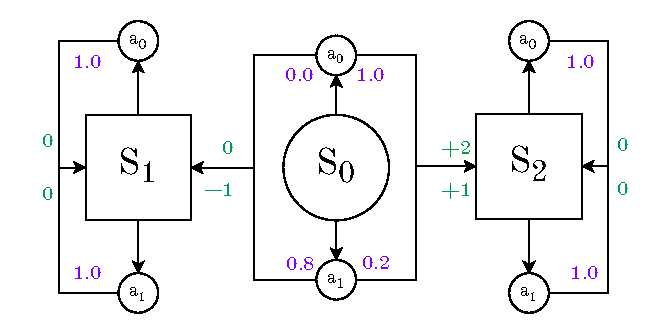
\includegraphics[width=1\linewidth]{diagrams/mdp.pdf}
    \caption{An example of a graphical representation of a Markov decision process. Squares depict terminal states. Transition probabilities are purple; rewards are green.}
    \label{fig:mdp}
\end{figure}

\subsection{Markov property}
Notice that the probabilistic transition function $p$ only takes the current state and action as inputs. Importantly, it does not take history into consideration. The probability of transitioning from state $s$ to state $s'$ using action $a$ is always the same no matter how the MDP got into the state $s$. This memorylessness of MDPs is known as the Markov property, and it is important to remember when implementing an environment since many RL algorithms rely on the environment to fulfill the Markov property. It can be formally defined as
\begin{equation}
P(S_{t+1}\mid S_t,A_t)=P(S_{t+1}\mid S_t,A_t,S_{t-1},A_{t-1}, \dotsc)
\end{equation}
An example of an environment that breaks this property could be the game of Pong\footnote{\url{https://en.wikipedia.org/wiki/Pong}} where the state is only the current frame. From just one frame, it is not possible to know in which direction or at what speed the ball will move after the next input. This can, of course, be easily fixed by including not only the position but also the speed and direction of the ball in the state (or using other techniques such as frame-stacking, where multiple frames are included in the observation). In real-world scenarios, fully capturing movement may require including higher-order dynamics like acceleration or jerk. However, in practice, modeling up to acceleration is typically sufficient for most RL tasks.

\subsection{MDP modifications}
It should be mentioned that there are many possible extensions for MDPs that could be necessary for representing actual environments, such as MDPs with continuous time, which do not operate on discrete time steps, or multi-agent MDPs, which allow multiple agents to interact with the environment at the same time.

One important extension is s partially observable MDP (POMDP). As mentioned earlier, in most cases, the agent does not receive the entire state of the environment it interacts with, but only some part of it -- an observation. To account for this, two more properties are added into the tuple defining the MDP -- $\mathcal{O}$ and $\epsilon$. $\mathcal{O}$ is the set of all possible observations -- an observation space. $\epsilon$ is a function $S \to \mathcal{D}(\mathcal{O})$ -- for a given state $s$ it returns a probability distribution over the observation space. However, to make things simpler, we will consider only regular MDPs for the rest of this chapter.

\section{Policy}
Now that the environment is formally defined using a MDP, we can also formally define the agent. We can imagine the agent as some entity that receives a state $s$ and, based on it, chooses an action $a$ that is then performed, and the agent receives a reward $r$ and a new state $s'$. As already mentioned, we call the tuple $(s, a, r, s')$ an experience. The entire chain of these experiences is called a trajectory $\tau$, and since the ending state of one experience and the initial state of the following experience is always the same, we can write it only once: $s_0,a_0,r_1,s_1,a_1,r_2,\dotsc \in (S\times A \times \mathbb{R})^{*}$. Note that a trajectory is infinitely long since even in a terminal state, we can still perform an action; it just won't give any reward or transition the environment into a different state. History is then some prefix of a trajectory ending in a state: $s_0,a_0,r_1,s_1,a_1,r_2,\dotsc, a_{t-1},r_t,s_t\in (S\times A \times \mathbb{R})^{*}\times S$. The agent has to make the decisions based on some rules. We call policy $\pi$ a function $\pi\colon (S\times A \times \mathbb{R})^{*}\times S \to \mathcal{D}(A)$, which returns a distribution over the action space based on the history up to that point~\cite[p. 19]{PA230}.

If we assume that the Markov property is fulfilled, we can simplify policy to just $\pi\colon S \to \mathcal{D}(A)$ because, in that case, the environment is memoryless, and thus, it does not matter how it ended up in the state $s_t$. Thanks to this, the agent (and its underlying policy) can be memoryless as well. Note that this is only true if the agent receives the entire state, so this simplification can not be applied to POMDPs (two different states might produce the same observation, and the history might be helpful to differentiate between them).

We can further simplify the policy by making it deterministic -- instead of returning a probability distribution $\mathcal{D}(A)$ it returns just a single action $a$. Such policy can be defined as just $\pi\colon S \to A$.

\section{The goal of RL}
\label{sec:goal}
Now that we have fully formally defined the environment (MDP) and the agent (policy), we can define the goal of RL. The goal is to find such a policy $\pi^*$ that maximizes the expected discounted cumulative reward, also referred to as the discounted return. The cumulative reward (or return) of a trajectory $\tau$ is defined as the sum of all received rewards:
\begin{equation}
G(\tau) = r_1+r_2+r_3+\dotsb = \sum_{i=0}^{\infty} r_{i+1}
\end{equation}
To get the discounted return, we exponentially decay the rewards by some discount factor $\gamma \in [0,1)$. This has two reasons. Since the trajectory can be infinitely long, if the policy found a cycle with a positive reward (even very small), it would lead to the cumulative reward being infinite. Second, it encourages policies that not only have the maximum reward but also get it as fast as possible because the reward will be less discounted. So, the discounted return $G$ on a trajectory $\tau$ with discount factor $\gamma$ is defined as:
\begin{equation}
G(\tau)=r_1+\gamma \cdot r_2+ \gamma^2 \cdot r_3+\dotsb = \sum_{i=0}^{\infty} \gamma^i\cdot r_{i+1}
\end{equation}
Finally, the expected discounted cumulative reward. As stated before, the environments are often stochastic -- they can start in many different states (with possibly different probabilities), and taking an action in a state can lead to different transitions (again with possibly different probabilities). Because of this, even a deterministic policy can have different trajectories on the same MDP each time, and those can, in turn, have different returns. Thus, it is important to find such a policy that will, on average, have the highest discounted return, not just in some specific single case.

\section{Value functions}

For a given policy $\pi$, we can calculate its value functions. These are functions that describe how this policy performs in some given environment. They can be used to compare policies with one another or used for learning purposes.

\subsection{State-value function}
\label{subsec:state_value_func}
The state-value function $v_\pi\colon S\to \mathbb{R}$ (often called just the value function) tells us the expected return of policy $\pi$ when starting in the state $s$.
\begin{equation}
v_\pi(s) = \mathbb{E}_\pi [G_t\mid S_t=s]
\end{equation}

If we know the underlying MDP, we can simply calculate it directly using the Bellman equation:

\begin{equation}
v_\pi(s) = \sum_a \pi(a\mid s) \cdot \sum_{s',r} p(s',r\mid s,a)\cdot[r+\gamma v_\pi(s')], \forall s \in S
\end{equation}

Due to the recursive nature of this formula, it would be quite hard to calculate directly, so in practice, an iterative algorithm that uses an already existing approximation for the next state is used (often called policy evaluation). When we do not have access to the MDP, we can use algorithms such as Monte Carlo or Temporal difference that repeatedly interact with the environment to collect experiences and then use this data to approximate the value functions.

\subsection{Action-value function}

Knowing how well the policy performs in a state can be useful, but it does not help it decide which action it should take (unless it also has access to the transition function). The action-value function $q_\pi\colon S \times A \to \mathbb{R}$ tells us the expected return of policy $\pi$ if the agent were to select action $a$ in state $s$ and then follow the policy until it reaches a terminal state.

\begin{equation}
q_\pi(s,a) = \mathbb{E}_\pi [G_t\mid S_t=s,A_t=a]
\end{equation}

Knowing the action-value function can help us improve the policy. Algorithms, such as Q-learning, and DQN, are based on this principle.

\subsection{Action-advantage function}

Lastly, the advantage function $a_\pi$ is a modification of the action-value function that tells us how much better (or worse) it is to take an action $a$ in a state $s$ compared to following the policy:

\begin{equation}
a_\pi(s,a) = q_\pi(s,a)-v_\pi(s)
\end{equation}

It does not really give us any new information compared to the action-value function (given we know the state-value function), but it allows us to compare the actions more easily.

\section{Exploration-exploitation tradeoff}
\label{sec:eplor-exploit}
As mentioned in Subsection \ref{subsec:state_value_func}, many RL algorithms rely on approximating a value function using an iterative algorithm and then use this information to improve the policy. To make the approximation, they need to repeatedly interact with the environment and collect experiences. To create the best approximation, it would be best to run the policy from every single possible state and try every single possible action, ideally, many times to account for randomness. Obviously, this is not feasible for any environments that contain more than a few thousand states, and it is outright impossible for environments with continuous state or action spaces.

Since exhaustive exploration is infeasible, RL algorithms must balance two competing objectives: discovering new strategies (exploration) and leveraging known good strategies (exploitation). This challenge is known as the exploration-exploitation tradeoff. Should we rather try completely new actions and risk wasting time on unproductive paths (explore), or stick to what we know works reasonably well, but risk completely missing some better strategies (exploit)? To measure how much of the training was \enquote{wasted} on exploring, we can use a metric called regret. To calculate regret $R$ at time $T$, we sum the differences between the expected reward given for the optimal action and the actual reward for the selected action for every step.

\begin{equation}
R(T) = \sum_{t=1}^{T}(\mathbb{E}[r^*]-r_t)
\end{equation}

Note that the optimal strategy must be known to calculate the expected optimal reward ($\mathbb{E}[r^*]$). If it is not known, other strategies must be used.

The goal is to find the optimal policy while maintaining the lowest total regret. To manage this tradeoff effectively, various exploration strategies have been developed. Below are three commonly used approaches:

\begin{itemize}
    \item (Decaying) epsilon-greedy exploration strategy -- given some constant $\varepsilon \in [0,1]$, choose a random action with the probability of $\varepsilon$; otherwise, choose the action currently estimated to be the best. More commonly, $\varepsilon$ is not a constant, but instead, it gets lowered (decayed) as training progresses.
    \item Upper confidence bound strategy -- when choosing which action to take next, a bonus is added to the estimates with lower confidences (those that are less explored). The bonus is calculated as $c\sqrt{\frac{\ln{t}}{N_t(a)+1}}$ where $c$ is some constant describing the importance of this bonus, $t$ is the episode number and $N_t(a)$ is how many times the action $a$ was already chosen (plus one to avoid division by zero).
    \item Softmax exploration strategy -- the chance of a certain action being selected is proportional to its action value estimate. To get the probabilities, we take the estimates and pass them through the softmax function, which will normalize them so that they are all between zero and one and their sum is equal to one. The softmax function is defined as $\sigma (v)_i = \frac{e^{v_i}}{\sum^{K}_{j=1}e^{v_j}}$ for the $i$-th value of a vector $v$ with $K$ elements. Of course, this would not work very well at the beginning when the estimates have high variance, so we also divided the estimates by a decaying hyper-parameter $\tau$ called temperature, which makes it so the estimates are less important at the beginning of the training.
\end{itemize}


\section{Reinforcement learning algorithms}
\label{sec:algos}

[TODO] tady by něco mělo být

\subsection{Value-based methods}

The simplest approach to reinforcement learning is learning to approximate the action-value function (either directly or calculating it using the state-value and advantage-value functions) and then using a greedy policy that selects the best action based on these approximations.

For simple environments with small discrete state and action spaces, it is possible to simply have a table of every state-action combination (tabular algorithms). There are many different algorithms utilizing this principle. They differ in the way they calculate the approximations (Temporal difference (TD), Monte-Carlo (MC), $\lambda$-TD), whether they use the same model for the approximation and exploration (SARSA, Q-learning), and in their exploration strategies. There are also some more advanced algorithms that approximate not only the Q function but also the underlying MDP to learn more efficiently (Dyna-Q).

While tabular algorithms can work very well for simple environments, they are unusable for any more complex environments. Even for just a $100 \times 100$-pixel binary image, this would require a table of over $10^{72247}$ numbers.

For these more complex environments, deep-learning is utilized; the approximator is a neural network whose loss function is calculated as the difference between the approximations and real values gathered during exploration. These methods often use a replay buffer -- a data structure that collects experience tuples from previous runs. When learning, examples are picked at random from this buffer, which somewhat minimizes the bias in data caused by the experiences from one episode not being independent. These methods include algorithms such as Neural Fitted Q-iteration (NFQ), Deep Q-Learning (DQN), and Double DQN (DDQN).

\subsection{Policy-based methods}

While value-based methods create policies indirectly based on a value function, policy-based methods learn the policy directly by outputting a probability distribution over actions. The learning is usually done by trying to maximize the probability of taking actions with a bigger advantage estimation using gradient ascent.

Purely policy-based algorithms are rarely used nowadays, but they are an important part of the actor-critic architecture introduced in the next subsection. Policy-based algorithms include REINFORCE and Vanilla Policy Gradient (VPG).

\subsection{Actor-critic methods}

Actor-critic methods combine both value-based and policy-based methods into one. They are composed of two parts: the actor and the critic. The critic is a value function estimator of the actor, which represents the policy by choosing the actions. The critic learns just like the value-based methods by minimizing TD or MC errors. The actor then learns by trying to maximize the expected return based on the value estimations provided by the critic.

Actor-critic methods combine the strengths of both value-based and policy-based methods. They are more stable, more sample efficient, and can deal with both discrete and continuous action spaces. State-of-the-art actor-critic algorithms include Twin Delayed Deep Deterministic Policy Gradient (TD3), Soft Actor-Critic (SAC), and Proximal Policy Optimization (PPO).

\chapter{RL in practice}

The previous chapter briefly explained the theory and terminology behind RL. This chapter follows up with an introduction to RL libraries and their usage. It should give enough context to make the source code of the experiments done in this thesis understandable.

As with most machine learning tasks, Python is the most popular programming language for RL, which is why I decided to use it in this thesis. AIVA is written mostly in .NET, but this should not be a problem since most machine learning libraries allow export into a common format such as ONNX\footnote{\url{https://onnx.ai/}} so that agents trained in Python can also be run natively in most other programming languages.

\section{Gymnasium}
\label{sec:gym}
Gymnasium\footnote{\url{https://gymnasium.farama.org/}} is a Python library that allows for easy creation of RL environments. It is a maintained fork of the Gym\footnote{\url{https://www.gymlibrary.dev/}} library developed by OpenAI. Its main purpose is to define a unified environment API, but it also contains many wrappers that simplify processes such as normalization, clipping, recording of the training, or vectorization of parallel training. It also provides many predefined environments that can be used to test new RL algorithms. The information in this section is from the official Gymnasium documentation~\cite{gym-docs}.

An environment is a Python class that inherits from the \texttt{Env} class. Inside the initialization method of this class, the observation and action space types must be defined. Gymnasium provides the following types of spaces:

\begin{itemize}
    \item \texttt{Box} -- represents a tensor ($n$-dimensional matrix of numbers) of a fixed shape. The numbers inside can be both bounded and unbounded. This type is useful for a representation of images or continuous actions.
    \item \texttt{Discrete} -- represents a space of finitely many integers. This is especially useful for discrete action spaces.
    \item \texttt{MultiBinary} -- tensor of boolean values.
    \item \texttt{MultiDiscrete} -- tensor of discrete values. 
    \item \texttt{Text} -- a string composed of specified characters.
    \item Composite spaces -- multiple fundamental spaces can be combined into a \texttt{Dictionary}, \texttt{Tuple}, \texttt{Sequence} of variable length, a \texttt{Graph} or a \texttt{Union}.
\end{itemize}

The environment class also requires the following methods to be implemented:

\begin{itemize}
    \item \texttt{reset} -- called to begin a new episode. It resets the environment to an initial state and returns the initial observation and a dictionary with auxiliary information for debugging or other purposes. It takes a seed value as an optional parameter.
    \item \texttt{step} -- performs a single time step of the environment. Its only input is the action decided by the agent, which has to adhere to the type defined in the initialization method. It transitions the environment to a new state, returning the new observation, the reward awarded for taking the action, whether the reached state was terminal, whether the episode was truncated (e.g. due to reaching a time limit), and again, a dictionary with auxiliary information.
    \item \texttt{render} -- a method for getting the current state of the environment in a human-friendly format. Each environment can define multiple render modes, one of which can then be selected during initialization. Most common formats include an RGB frame, text, or a list of RGB frames. This method can be either called manually by a user or, more often, by a monitoring wrapper of the environment.
    \item \texttt{close} -- a clean-up method. Should close render windows, end database connections, etc.
\end{itemize}

Once an environment is defined, it should be registered using the \texttt{gymnasium.envs.registration.register} function, which allows it to be later created using the \texttt{gymnasium.make} function. Such an environment can then be wrapped in the aforementioned wrappers and passed to a RL algorithm.

\section{Stable-Baselines3}
Stable-Baselines3\footnote{\url{https://stable-baselines3.readthedocs.io/en/master/}} (SB3) is a Python library containing implementations of RL algorithms. It originated as a maintained fork of the OpenAI Baselines\footnote{\url{https://github.com/openai/baselines}} library but has since evolved to include numerous additional algorithms, an improved API, and comprehensive documentation. The algorithms are implemented using PyTorch, which allows for simple modifications of the underlying neural networks. These algorithms interact with environments defined using the Gymnasium API described in Section~\ref{sec:gym}. The information in this section is from the official SB3 documentation~\cite{SB3-docs}.

To create a new model, one instantiates a class provided by SB3 (such as \texttt{PPO}, \texttt{A2C}, or \texttt{DDPG}) and supplies the environment along with additional parameters, including hyperparameters, GPU selection, and logging options. The library also supports saving and loading models via the \texttt{save} and \texttt{load} methods.

Once a model has been created, it can be trained using the \texttt{learn} method, which trains the model for the provided amount of time steps. Additionally, a callback can be passed as well. Callbacks are special classes that can call functions when certain events happen during training. For example, the \texttt{EvalCallback} evaluates the model every $n$ episode and can additionally save the model on the new best mean reward. SB3 also provides an API for creating custom callbacks.

Inference on a model is done through the \texttt{predict} method, which returns the model's decided action for a given observation.

I chose to use this library over others mainly because it contains algorithm implementations, simple-to-use API, and good documentation. I chose not to implement the algorithms on my own since they would probably perform worse, and it is unlikely that these implementations would change the outcome of this thesis.

\section{Optuna}
\label{sec:optuna}

Optuna\footnote{\url{https://optuna.org/}} is an open-source framework used for automated hyperparameter search (or, in general, for optimizing any function with parameters). It uses state-of-the-art algorithms to suggest hyperparameters based on previous experiences, making it much more time-efficient than usual methods such as grid search. Once again, the information in this section is sourced from its official documentation~\cite{optuna-docs}.

Optuna can optimize any objective function. Such function takes a \texttt{trial} object as an input, uses its methods like \texttt{trial.suggest\_int} or \texttt{trial.suggest\_categorical} to get the suggested hyperparameters and returns a float representing how well the objective was met (this is most often some accuracy metric, in the case of RL, it is the mean episode reward). A study is then created using the \texttt{optuna.create\_study} function. This study can then be optimized for some amount of trials, after which it returns the best found hyperparameters.

A study can be connected to a relational database that stores previous trails. The results can then be visualized using Optuna Dashboard\footnote{\url{https://optuna-dashboard.readthedocs.io/}}. It plots information such as hyperparameter importance, the tuning progression, and much more.

It is also possible to run multiple Optuna instances in parallel, all using the same database. This allows for a very simple way of distributed tuning on multiple machines with almost linear scaling.

If the objective function is capable of producing intermediate values, Optuna can also be configured to prune attempts that are unlikely to beat the current best attempt, which can speed up the process significantly.

\section{Hardware}

Most state-of-the-art RL algorithms are based on deep learning. To train large neural networks in a reasonable time, powerful enough hardware is needed. Most of the experiments in this thesis were done on my personal computer (Intel i5-12400, NVIDIA RTX 3080). For long-running trainings, I used one of Y Soft's GPU nodes (AMD Ryzen 9 5950X, NVIDIA RTX A4000). The speed of these two machines is very comparable in a single environment, but the 16 cores of the AMD Ryzen 9 5950X significantly outperform the Intel i5-12400's 6 cores in vectorized environments.

\chapter{Experiments}

\section{Defining the problem}
\label{sec:problem_definition}

Before we start training models, it is important to define the problem we are trying to solve first. The goal is to create an algorithm that receives an image as input (be it directly a screenshot of a website or some preprocessed version to simplify the task). It outputs a set of bounding boxes, each of which is a bounding rectangle of an object in the image.

With regular supervised learning solutions, one of the biggest challenges of this sort of object detection is the variability of the output size. Each image can contain a different amount of objects. Thankfully, this is not an issue for RL, as it is naturally sequential with different episode lengths. We need the agent to perform actions that somehow represent a bounding box (be it a one-to-one relationship where each action is one selection or a many-to-one relationship where multiple actions combined create a selection). Since we want to satisfy the Markov property the agent can not remember which objects were already detected. Because of this we have to somehow modify the state to contain this information.

First, we have to decide on the state and action spaces and the representation of the states and actions. I decided to start with the simplest mapping I could think of; the input of the algorithm is an image that can be used directly as the state. More formally, the input type will be represented by a tensor of size $C\times M \times N$ where $C$ is the channel count (3 for RGB images, 1 for grayscale and binary images), $M$ and $N$ are the width and height of the image. The values are bounded to 0-255, or 0-1 after normalization. For this, we can use the \texttt{Box} Gymnasium type. In theory, the \texttt{MultiDiscrete} could be more suitable as the values are discrete, not continuous, but SB3 does not currently support using convolutional layers on discrete spaces.

The representation of actions is a bit more complicated. At first, I again chose the simplest mapping, where each action is one selection; later on, I also tried a different approach. Each action is four floating point numbers from 0-1. The first two numbers represent the $x$ and $y$ coordinates of the selection's center and the other two are the width and height. Again, there are more possible options, such as the coordinates of two corners; again, these are discussed later. Such action space can also be defined using the \texttt{Box} Gymnasium type.

\section{Choosing an algorithm}
As discussed in Section \ref{sec:algos}, there are many different reinforcement learning algorithms. The Stable-Baselines3 library implements a total of seven: \texttt{A2C}, \texttt{DDPG}, \texttt{DQN}, \texttt{HER} (in newer versions of SB3 it is no longer a separate algorithm but a type of replay buffer), \texttt{PPO}, \texttt{SAC} and \texttt{TD3}. Of course, the algorithm is one of the things we can change and experiment with, but we have to choose one to start with.

I decided on \texttt{PPO} mainly through a process of elimination. First of all, \texttt{TD3} is an improvement of \texttt{DDPG} and \texttt{PPO} is an improvement of \texttt{A2C}. It is unlikely that the simpler version would perform better, so we can eliminate them. As stated, the action space is continuous, which eliminates \texttt{DQN}. Next up, the state is an image. Even a binary image of $100\times100$ pixels requires over a kilobyte of memory. This makes algorithms that utilize a replay buffer quite impractical, especially if we want to have room to increase the image size later on. This eliminates \texttt{HER}, \texttt{SAC} and \texttt{TD3}, leaving us only with \texttt{PPO}.

\texttt{PPO} is also the recommended algorithm for continuous actions when multiprocessing is available according to the SB3 documentation \cite{SB3-docs}.

\section{Custom environments}
It might be tempting to start training in an environment that simulates the final problem. When I initially attempted this approach, the results were unsatisfactory, as expected. The complexity of the setup made experimentation difficult: if a change in parameters led to equally poor results, it was unclear whether the adjustment was ineffective, or if the state of the system was so far from ideal that even a beneficial change wouldn't have a noticeable effect. So, instead, I started with a very simplified version of the final problem, and once I reached satisfactory results, I moved on to a more complex task until hopefully eventually returning to the final environment with enough knowledge to complete it.

This also allowed for transfer learning and curriculum learning. I could train a model on a simpler version of the problem and then fine-tune it on a more complex one. It is more likely that a model that can find rectangles will be able to learn to find other shapes than a model that does not know anything.

The following sections talk about the intermediate environments in greater detail and also provide information on all the steps and experiments I took in order to solve them.

\section{Static square of uniform size}
% env v0 %
The very simplest problem I could come up with that at least somewhat resembles the real problem is the following.
\begin{itemize}
    \item State: consists of a black $100\times100$ pixel image with a white square in the middle. The position of this square is always the same between episodes, and its size does not change. An example can be seen in figure \ref{fig:env0}
    \item Action: the model returns four numbers representing the bounding box ($x$ and $y$ coordinates of the center and the width and height). The action has no effect on the state. It only gives a reward. The state does not change since the episode is always one step long.
    \item Reward: The reward is calculated using the Intersection over Union (IoU) metric (area of the intersection of the correct bounding box compared to the guess divided by the area of their union). When the bounding boxes do not overlap at all, IoU is always zero, no matter how far away they are. In those cases, the reward is the negation of the distance of the centers of the bounding boxes.
    \item Algorithm: \texttt{PPO} with the default \texttt{CnnPolicy} provided by SB3 (the architecture is shown in figure \ref{fig:cnn_policy} in appendix), default hyperparameters.
\end{itemize}

\begin{figure}
    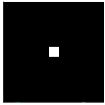
\includegraphics[width=0.5\linewidth]{env_examples/env0.png}
    \caption{Example of the simplest environment with a static square. TODO: udělat lepší obrázek než screenshot}
    \label{fig:env0}
\end{figure}

I expected the model to overfit very quickly since the state was always identical, and there was a single action that always yielded the best possible reward. The model got to an IoU of 0.94 after around 160,000 time steps, but surprisingly, it started to critically forget quite quickly after that, and it never recovered. Nonetheless, the environment was successfully solved. Since this behavior happened less and less for the more complex environments, I assume that the problem was too simple for a complex algorithm such as \texttt{PPO}.

Figure \ref{fig:v0_rew} shows the mean reward per episode during the training. Since an episode always consists of exactly one observation, the biggest possible reward is 1 (since that is the highest score of IoU). The $x$-axis shows the elapsed time steps.

\begin{figure}
    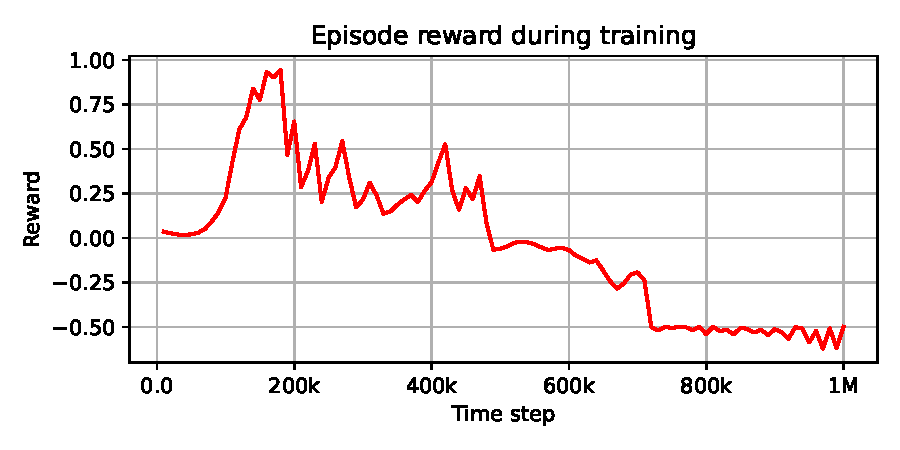
\includegraphics[width=1\linewidth]{graphs/v0.pdf}
    \caption{The mean reward per episode for the simple static square environment. The data was collected by evaluating the agent for 20 episodes after every 10,000 training time steps.}
    \label{fig:v0_rew}
\end{figure}

\section{Moving square of uniform size}
% env v1 %
The next step forward was to make the square move. The initial state was created by randomly choosing a position within the image and placing the square there. All the other options (reward, action, and algorithm) remain the same. Some examples of this environment can be seen in figure \ref{fig:env1}.

\begin{figure}
    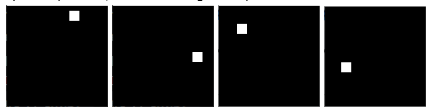
\includegraphics[width=1\linewidth]{env_examples/env1.png}
    \caption{Four examples of the environment with a moving square. TODO: make look good, not screenshot}
    \label{fig:env1}
\end{figure}

The best model was able to guess the position of the bounding box pretty well, usually within the actual square, but it struggled with the size even though, again, I expected it to overfit since there was a single correct answer. It even sometimes predicted the width or height of zero, even though that always resulted in a zero reward. Just like the previous model, this one also started to catastrophically forget. Even though the result was not perfect, it showed that the model could deal with the movement, so I decided to continue.

\section{Single moving rectangle}
% env v2 %
\label{sec:moving_rectangle}
The next environment was, once again, very similar, the only exception being that the object could now have any size, not just a perfect square of uniform size. Both the placement and size were chosen randomly but with a few constraints. The rectangle could not have a width or height of less than 10 percent of the image, and it could not overflow outside of the image. A few examples can be seen in Figure \ref{fig:env2}.

\begin{figure}
    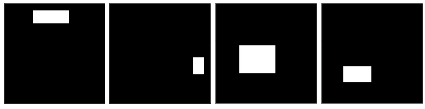
\includegraphics[width=1\linewidth]{env_examples/env2.png}
    \caption{Four examples of the environment with moving rectangles TODO: make look good, not screenshot}
    \label{fig:env2}
\end{figure}

This time, I also wanted to try the other network architecture provided by the SB3 library \texttt{MlpPolicy}, which has a simpler, non-CNN-based architecture (shown in detail in Figure \ref{fig:mlp_policy} in the appendix). It is simpler (1.3 million parameters compared to 2.7 million), but for such a simple problem, that could still be more than enough.

The MLP policy actually outperformed the CNN, and it also seemed a lot more stable. While it had some dips in its performance (probably caused by exploration), it always recovered and did not critically forget, as visible in figure \ref{fig:v2_mlp_cnn}.

\begin{figure}
    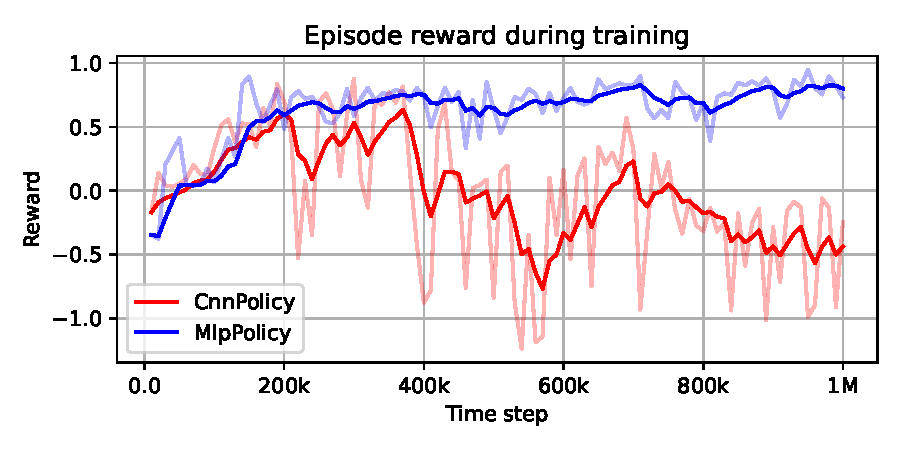
\includegraphics[width=1\linewidth]{graphs/v2_mpl_cnn.pdf}
    \caption{Comparison of the mean reward of the MLP and CNN policies. The data was collected by evaluating the agent for 20 episodes after every 10,000 training time steps. Both the raw values and an exponential moving average are shown for better clarity.}
    \label{fig:v2_mlp_cnn}
\end{figure}

\section{Multiple rectangles}
\label{sec:multi-rect}
% env v3 %
Since the performance of detecting a single object seemed pretty good, the next logical step was to add more objects. The next environment had the following properties:
\begin{itemize}
    \item State: consists of a black $100\times100$ pixel image. Five attempts are made at placing a rectangle of a random size in a random place. If it does not overlap with any already placed rectangle, it is added to the image. Because of this randomness, the amount of objects changes between episodes; it can be anywhere between 1 and 5, but on average, 3.5 objects are placed. Four examples can be seen in Figure \ref{fig:env3}.
    \item Action: the model returns 4 numbers representing the bounding box ($x$ and $y$ coordinates of the center and the width and height). If the predicted bounding box overlaps with any of the objects, that object is erased from the state (in its entirety, even if the prediction does not cover all of it).
    \item Reward: The reward calculation is very similar to the previous environments. If the prediction overlaps any objects, their IoU is the reward (if it overlaps multiple, then the maximum IoU is given). The episode is terminated when all objects are removed or stopped after $n$ guesses, where $n$ is the starting amount of objects. Note that the model is not directly punished for selecting more than one object, but since only one reward is given, it is more beneficial to select them separately since, otherwise, the other object is lost without any reward.
\end{itemize}

\begin{figure}
    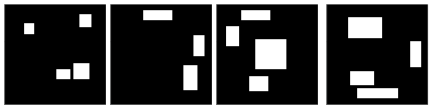
\includegraphics[width=1\linewidth]{env_examples/env3.png}
    \caption{Four examples of the environment with multiple moving rectangles}
    \label{fig:env3}
\end{figure}

Again, I tried both MLP and CNN strategies. This time, they both performed very similarly, stabilizing at a mean reward per episode of around 0.75 after around 400,000 time steps. At first glance, the results might seem just as good as in the previous environment, but remember that since the episodes last multiple time steps (3.5 on average), the results are pretty poor as the maximum possible reward per episode is now around 3.5, whereas before, it was just 1. This was despite both agents doing an average of 3 actions per episode.

\subsection{Different action definition}

As mentioned in Section \ref{sec:problem_definition}, there are multiple ways to define a bounding box using four numbers. Before, the action was defined as $(x, y, w, h)$. In this experiment, I changed the meaning to $(x_1, y_1, x_2, y_2)$ or the coordinates of the top-left and bottom-right corners. My thought process was that since convolutions are translation invariant but not scale invariant, it should be easier to find the corners than the entire object whose size is variable.

This did improve the performance of the CNN-based model slightly (from 0.75 to 1) but surprisingly made the MLP-based model worse (from 0.75 to 0.5).

\subsection{Transfer from previous environment}

Since the previous environment used the same definition of space and actions, it was possible to reuse its weights in this environment with the potential of transferring some of the learned knowledge. While the transferred agent did start off much better, it quickly forgot everything and did not catch up to the agent initialized with random weights.

\subsection{Changing the network architecture}
\label{subsec:arch_change}

The graphs of all of the previous experiments in this section showed a similar trend. They started off learning relatively quickly, making great progress. After the first 200,000 time steps, the progress slowed down dramatically. This could hint at the agent being too simple for the environment and not being able to learn it.

Since SB3 is based on PyTorch, it is relatively simple to modify the underlying neural networks. In the default \texttt{CnnPolicy}, the actor and the critic share a feature extractor with three convolutional layers and one fully connected layer. Then, each of them has a single fully connected layer (for more detail, see Figure \ref{fig:cnn_policy}).

I modified the architecture by adding an extra fully connected layer to the feature extractor and two extra fully connected layers to both the actor and the critic. This meant that the model had around 6 million parameters. The new architecture can be seen in detail in Figure \ref{fig:bigger_net_policy} in the appendix.

This change helped quite a bit. It outperformed the simple networks, and it continued learning even after more than 7 million episodes. Figure \ref{fig:v3_bigger_net} shows the comparison between the bigger network and the best CNN policy model. The mean episode lengths did not differ dramatically.

\begin{figure}
    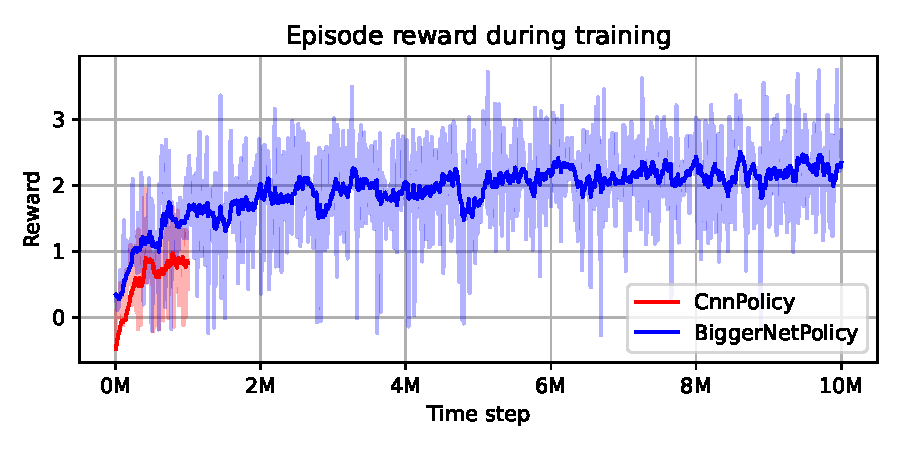
\includegraphics[width=1\linewidth]{graphs/v3_cnn_vs_biggernet.pdf}
    \caption{Comparison of the mean reward of the default \texttt{CnnPolicy} and a bigger network. The data was collected by evaluating the agent for 20 episodes after every 10,000 training time steps. Both the raw values and an exponential moving average are shown for better clarity.}
    \label{fig:v3_bigger_net}
\end{figure}

The resulting model took around 6 hours to train and reached a mean reward of around 2.1 per episode or an average IoU of 0.6. While this might still sound pretty bad, note that especially with smaller objects, IoU is pretty strict. For example, if for a rectangle of size $20\times 20$, we guessed a bounding box of the correct size but shifted to the left and down by 2 pixels, the IoU would be only 0.68 even though the guess is only off by 10 percent. Another problem that brings the average down is that sometimes, when the image contained two objects far apart, the model got confused and predicted a bounding box between them repeatedly until the episode was stopped; an example of this behavior can be seen in Figure \ref{fig:v3_stuck}.

\begin{figure}
    \centering
    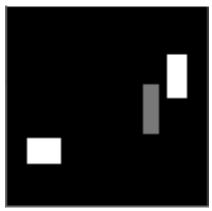
\includegraphics[width=0.5\linewidth]{results/v3_stuck.png}
    \caption{Example of the model getting stuck when two objects are far apart. White rectangles are the actual objects, and grey is the prediction.}
    \label{fig:v3_stuck}
\end{figure}

\section{Different shapes}
%v4 env%
Now that the model was able to locate multiple rectangles in a single image with quite 
 a good accuracy, the next step was to introduce other shapes as well. This new environment was identical to the previous one, but instead of just rectangles, there could also be ellipses and triangles. Since the rules were still the same, there were an average of 3.5 objects, and their bounding boxes did not collide. Some examples of this environment can be seen in figure \ref{fig:env4}.

\begin{figure}
    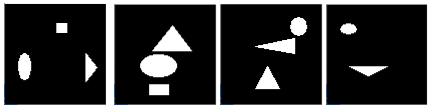
\includegraphics[width=1\linewidth]{env_examples/env4.png}
    \caption{Four examples of the environment with multiple different objects}
    \label{fig:env4}
\end{figure}
 
The training on my bigger network started off very similarly to the previous environment, but it never reached quite the same results, stopping at a reward of around 1.5.

Since the problem is similar to the previous one, I again tried to use transfer learning with the best model from the previous environment for the new one. It actually started with very good results and stayed at a reward of around 2.0 for the rest of the training, only improving a little bit.

This showed me that it was definitely possible to get good results. But I wanted to avoid transfer learning, if possible, until the very end because if it were needed this early on, it would create a very long and impractical chain of models that depend on one another. For those reasons, I wanted to improve the network further.

\subsection{ResNet-18 feature extractor}
\label{subsec:resnet}

It is a common practice not to create your own feature extractor but instead to use an already existing convolutional network trained on a similar problem, remove the fully connected layers, and use the rest as a feature extractor \cite[p. 256]{DLforVisualSystems}. I wanted to try this approach.

ResNet is a model architecture first proposed in the paper \textit{Deep Residual Learning for Image Recognition} \cite{ResNet18}. It introduced multiple sizes of the architecture, such as ResNet-18, ResNet-34, ResNet-50, and more. I decided to try the smallest one since even that would be a significant upgrade over the current feature extractor. The architecture of ResNet-18 can be seen in Figure \ref{fig:resnet}.

\begin{figure}
    \centering
    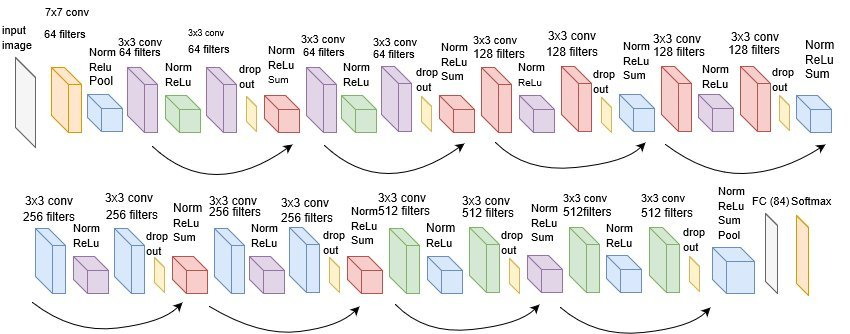
\includegraphics[width=1\linewidth]{diagrams/resnet.png}
    \caption{Architecture of ResNet18. The illustration was taken from \cite{resnet_illustration}. TODO možná si udělám vlastní obrázek, tenhle je hnusnej}
    \label{fig:resnet}
\end{figure}

It contains 18 convolutional layers (hence the 18 in the name), each followed by a batch normalization layer and some by a dropout layer. An important feature of ResNet are skip connections, which help with vanishing gradients. The PyTorch implementation ends with an adaptive average pooling layer. Unlike regular pooling layers, it has the output size as a parameter and chooses the stride and kernel size automatically based on the input. This makes it so that the output has the same size regardless of the input size

A slight complication is that ResNet-18 is meant for colored images (3 channels), but we are currently using binary grayscale images (1 channel), although this might change in the future. There are multiple ways of solving this problem; the simplest is to just duplicate the one channel 3 times. I did something a bit different, adding a convolutional layer at the beginning with a kernel of size $1\times1\times3$, which creates 3 feature maps from our one image. This is very similar to just duplicating the channel 3 times, but the kernel contains learnable parameters, so it is possible for the channels to be different if the network finds that useful. The entire architecture is shown in figure \ref{fig:resnet_arch} in the appendix.

It is also important to note that the ResNet-18 provided by PyTorch was pre-trained on the COCO dataset, which consists of photographs. This could mean that the knowledge won't transfer that well for binary images (and later on images of websites).

I tried again on the same environment. At first, I used the weights from PyTorch, and I froze them because I thought this would speed up the training. The results were very poor. Next, I ran the same test, but this time, the weights were no longer frozen and could thus adapt to the new problem. This time, the training went much better, reaching a reward of around 2.8 in less than 2.5 million time steps. Lastly, I also wanted to test whether the pre-trained weights made any difference compared to randomly initialized weights. The comparison of these three experiments and the best result reached with the previous architecture can be seen in Figure \ref{fig:v4_resnet_graph}. 

\begin{figure}
    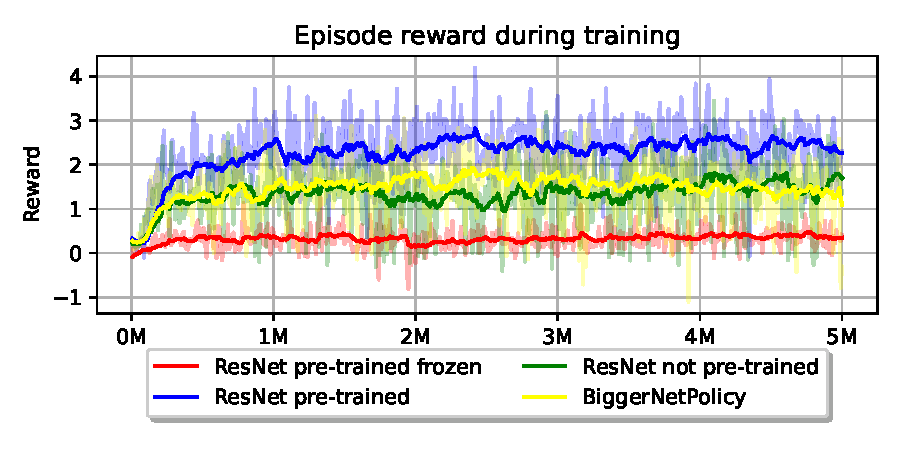
\includegraphics[width=1\linewidth]{graphs/v4_resnet_graph.pdf}
    \caption{Comparison of the mean reward of the pre-trained frozen, pre-trained fine-tunable, and not pre-trained ResNet-18 based agents with the previous architecture. The data was collected by evaluating the agent for 20 episodes after every 10,000 training time steps. Both the raw values and an exponential moving average are shown for better clarity.}
    \label{fig:v4_resnet_graph}
\end{figure}

While the improvement in performance was great, it also slowed down the training significantly. It took around 2.5 hours for one million time steps, which is around three times slower.

\section{Hollow shapes}
%env 5%
One big simplification we are currently undertaking is, that each position in the image can belong to at most one object, which is not the case in the real problem. To be able to put one object inside others, we need to mark only its edge; otherwise, the inside object will not be visible. In this next environment, the only change is the objects being just their outlines as visible in figure \ref{fig:env5}.

\begin{figure}
    \centering
    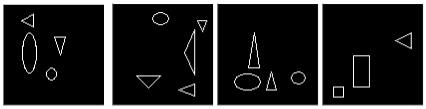
\includegraphics[width=1\linewidth]{env_examples/env5.png}
    \caption{Four examples of the new environment}
    \label{fig:env5}
\end{figure}
 
This change had little to no effect on the training progression.

\section{Bigger images}
Poznámka: Možná tuto sekci vynechám, jakože jsou tam I zajímavý věci, ale ve výsledku jsem to pak už moc nepoužil.
%env 6%
At this point, I was working with images of size $100\times100$ pixels, whereas AIVA currently uses a resolution of $1920\times1080$ pixels. Since we only need to locate the objects, which should not require pixel-sized details, some downscaling is possible, but squashing the image all the way down to $100\times100$ pixels would likely be too much. Because of this, I wanted to experiment with larger image states.

Thanks to the aforementioned adaptive average pooling layer used in the ResNet feature extractor, changing the image size would not require any large modifications of the network architecture.

Due to hardware limitations (GPU memory), the biggest image size that I was able to get running was $640\times480$ pixels, but even then, the training speed slowdown was so significant that I decided not to be so ambitious and I continued with an image size of $200\times200$ pixels (this slowed down the training around two times).

The size increase itself did not cause any big differences in the training except for the speed. But since the image was bigger it also allowed for more objects to be placed (7 on average). Unfortunately, the reward per object dropped significantly. The model learned to place large bounding box predictions in relevant areas. This did result in a positive reward most of the time but was far from optimal since it usually removed multiple objects at once. The likely cause was that the current reward function did not punish selecting multiple objects at once directly. I came up with two new ways, to calculate the reward in the case where the guess bounding box intersects multiple objects:

\begin{itemize}
    \item Find all objects that intersect with the guess. Find the object with the biggest overlap and calculate its IoU. Calculate the sum of the overlap areas of all the other intersecting objects with the guess, divide this sum by the guess' area, and subtract this from the IoU.
    \item Calculate IoUs of all the objects that intersect with the guess. The reward is the biggest IoU minus the sum of all the other IoUs multiplied by a constant.
\end{itemize}

The first option did help, bringing the per-object IoU from 0.5 to around 0.6. The second one had a very minimal impact. While IoU of 0.6 is usually considered acceptable \cite[p. 291]{DLforVisualSystems}, this experiment showed me that my current solution had problems even with an object count of less than 10, which is not acceptable since an average website probably contains closer to 100 objects.

\section{Hierarchical environment}
\label{sec:hierarchical-env}

So far all the environments comprised of objects that did not intersect in any way. They were completely independent, and thus, the order in which they were selected did not matter at all. This, of course, differs from how real websites look. They have a hierarchy of objects (one object can contain many others). The next step was to create an environment that would represent this more faithfully.

At first, I tried to use the same technique as before -- randomly attempting to place objects that do not overlap, but this time, I allowed such overlaps where one object was fully inside another. This did not work very well; the number of objects differed greatly between attempts, they were often placed very close to one another, and the depth of the hierarchy was very shallow. So, instead, I created a generator that directly created a tree-like structure. It starts with a root object that encloses the whole image, then it selects an area inside with a random offset to the parent object and randomly selects the number of children, their sizes, and the spacing between them. The algorithm then does this recursively for each child. It is also possible to customize the maximum depth, the minimum size of an object, minimum spacing, and so on. Some examples of this new generation can be seen in figure \ref{fig:env7}

\begin{figure}
    \centering
    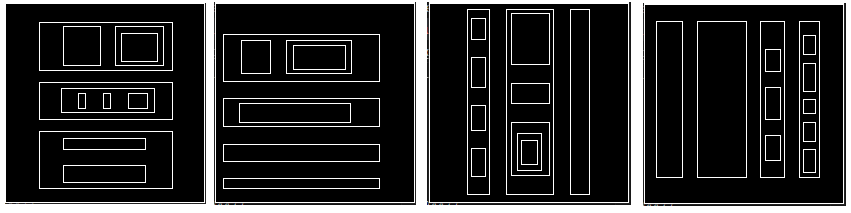
\includegraphics[width=1\linewidth]{env_examples/env7.png}
    \caption{Four examples of the new environment}
    \label{fig:env7}
\end{figure}

A new reward function was needed as well. I came up with the following method. First, find all objects that the guess intersects with or fully encloses; if there are none, also include objects that fully enclose the guess (there will always be at least the root). If there is just one such object, the reward is the IoU of this object with the guess minus the percentage of its area occupied by its children that have not been guessed yet (this is to discourage selecting objects that still have children). This object is then removed (including all of its children). If there are multiple intersecting objects, then the one that is deepest in the hierarchy is chosen, and the same calculations are done. The episode ends when the root object is removed.

I tested this new environment by training two new models. One from scratch and the other transferred from the previous environment. After around 7 million time steps, they both managed to get an average reward of about 2. The transferred model did perform slightly better but not by much. From the testing, it was clear that the model learned that placing long bounding boxes of width zero would almost always result in a nonnegative reward because the IoU of such bounding box is always zero, and the model did not explore enough to realize that it could do much better.

\subsection{Manual hyperparameter tuning}

One thing I have not yet experimented with was hyperparameter tuning. Since I needed to encourage the model to explore more, this was a perfect opportunity. I manually tried changing each of the following parameters:

\begin{itemize}
    \item The discount factor $\gamma$ (described in Section \ref{sec:goal}) -- By default, this parameter is set to 0.99, but in our case, discounting does not really make sense. Because of how the environment is set up, the maximum number of steps for the episode is capped, and an ideal policy will use up all of them. Thus, discounting is not needed, and $\gamma$ should be set to 1.
    \item Entropy loss coefficient $c_2$ -- The PPO loss function contains an entropy bonus that rewards less deterministic policies. Increasing it should thus lead to a more stochastic model and more exploration~\cite{PPO_paper}. By default, this hyperparameter is set to 0.
    \item Clipping range $\epsilon$ -- One of the main benefits of PPO is its clipping function that prevents big updates to the policy and value function, which should prevent it from \enquote{jumping off a cliff}~\cite{PPO_paper}. By increasing it, the training might become more unstable, but it also might help to get out of local maxima.
    \item Learning rate $\varepsilon$ -- When making an update to the policy network, the gradient is multiplied by this constant. Higher learning should make the training faster, but at the same time, the jumps are bigger, which can lead to unstable learning.
\end{itemize}

I tried both lowering and increasing each of these parameters, but unfortunately, none of the changes had a bigger positive impact. Lowering $\gamma$ and increasing the clip range did lead to slightly better results, but only by a little.

Later, when I discovered Optuna (see Section \ref{sec:optuna}), I also attempted an automated hyperparameter search, but even that did not lead to much progress. Since I did not have many ideas left on how to improve the training further, I decided to try a completely different approach.

\section{Switching to discrete actions}
\label{sec:iterative}

Since the results of the previous approach, which guessed bounding boxes directly (one action = one prediction), did not work well, especially in a more complex environment, I wanted to try a different approach. \cite{rl_object_detection}~describes and compares two approaches for object detection using reinforcement learning, both using discrete action space. Both of these methods start with a bounding box spanning the entire image, and the agent chooses actions to modify this selection repeatedly until it is happy with the prediction, at which point it selects the \texttt{trigger} action, which ends the episode and grants the final reward.

The first method, originally described in~\cite{hierarchical_od_with_drl}, has five movement actions (each resulting in zooming towards one of the corners or the center of the image) and a stop action. It showed promising results on a single object, single class object detection, but it is unusable for our purpose since it only produces bounding boxes with the same aspect ratio as the image.

The second method, originally described in~\cite{iterative_od_with_rl}, uses a similar approach, but instead of five actions for zooming in different areas, it has a total of eight movement actions (plus the trigger), four of which move the bounding box (up, down, left and right), two for size changes (zoom in, zoom out) and two for aspect-ratio changes (making the box fatter or taller). This allows for way more flexibility, although some bounding boxes are still impossible because the changes are of some fixed size, but if this size is small enough, it should be fine as we do not need pixel-perfect predictions. An example of one episode can be seen in figure \ref{fig:exmaple_from_paper}.

\begin{figure}
    \centering
    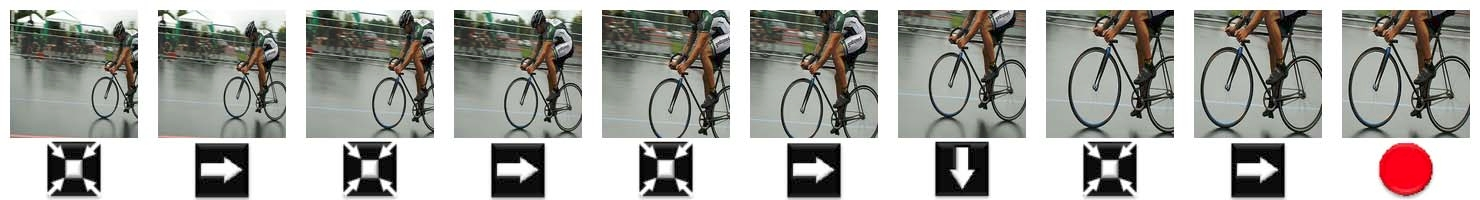
\includegraphics[width=1\linewidth]{diagrams/45.jpg}
    \caption{Example of taken actions to locate and object~\cite{iterative_od_with_rl}}
    \label{fig:exmaple_from_paper}
\end{figure}

As for the observation space, it is once again an image, but this time only the part that is inside the current bounding box scaled up to some fixed size since regular RL algorithms do not allow for an input of variable size. The original paper~\cite{iterative_od_with_rl} also used a vector of ten previous one-hot encoded actions, but~\cite{rl_object_detection} found that including them did not help.

I implemented a simpler version of this approach with only four actions, each of them shrinking the bounding box by some fixed percentage from one of the four sides. This simplifies the problem while keeping the ability to create predictions of any size.

The suggested reward function compares the IoU of the state before and after an action is taken and gives a reward of +1 if the action improved the guess and -1 if it got worse. When the trigger action is taken, a reward of $\eta$ is given if the resulting IoU is over some threshold $\tau$, $-\eta$ otherwise. The suggested values are $\eta=3$, $\tau=0.5$. \cite{rl_object_detection}~further tried changing them but did not find any improvements when they were increased.

This reward function is good for single object detection because the correct action will always improve the IoU, but when multiple objects are present, and the calculation is more complicated, this does not have to be the case. For this reason, I started my experiment with a much simpler sparse reward function, which only gives a reward for the trigger action. The reward is computed using the same calculation as in my previous environments.

\section{Single moving rectangle with discrete actions}

To test this new approach, I modified the environment described in Section \ref{sec:moving_rectangle}, which contains just a single rectangle. The model learned to find the rectangle pretty quickly, but the accuracy was not great, mainly because the selection shrinking was too large (one step shrunk the bounding box by 15 \%). When I lowered it to just 5 \%, the accuracy improved, but it took way too many steps (around 60), which would later slow down the inference by a lot.

Compared to the previous approach on the same environment, the training did take around ten times as many time steps to get to the same reward, but this was expected since suddenly a single guess required 30 to 50 time steps instead of just one.

\section{Multiple rectangles with discrete actions}

Since the results in the simple single-rectangle environment were satisfactory, I continued and modified the environment described in Section \ref{sec:multi-rect} to also use discrete actions. To account for the problematic accuracy caused by too large steps shown in the previous environment, I implemented two actions per direction, one shrinking the bounding box by 15 \% and one by just 2.5 \%. This does make the task slightly more complex but, at the same time, allows for precise predictions with a low amount of steps.

This is the environment where, with the previous approach, I had to switch to the bigger network. This time, I went directly with the ResNet-18-based network. This combination worked really well, reaching the same reward of 2.1 in only around 700,000 time steps compared to the 10,000,000 with the previous approach, even though one episode took around 80 time steps compared to 3.5.

\section{Hierarchical environment with discrete actions}

Seeing the great success of the new approach, I decided to skip all the way to the hierarchical environment described in Section \ref{sec:hierarchical-env}, which I was not able to solve using continuous actions.

\subsection{Changing to dense reward function}

Unfortunately, even this time, the results were terrible. The agent struggled to even reach the positive reward. Since the actions described in \cite{iterative_od_with_rl} were helpful so far, I also wanted to get closer to their reward function. The main change was going from a semi-sparse function (only giving rewards for trigger actions) to a dense function (rewarding every action). This should give the agent a lot more information to learn from.

I came up with the following. After each interaction find all leaf elements (with no children) that have an overlap with the current selection. If there are none, reward zero. Otherwise, find the element that has the highest IoU with the current selection. If the selected action is the trigger action and the IoU is over 0.5, reward 3, else -3. If it is not the trigger action, compare the IoU with the IoU after the previous action and reward the difference.

After some experimenting, changed the reward function for the trigger action not to give a fixed constant value but instead award 3 times the selection IoU since otherwise there would be little incentive to go past the threshold IoU of 0.5.

\subsection{Automated hyperparameter tuning}

Since I was not seeing much progress, I decided to revisit hyperparameter tuning once more, but this time not trying to find them manually but instead using Optuna (see Section \ref{sec:optuna}).

I ran a study of 200 trials, each running 200,000 time steps (if not pruned earlier). This took around 24 hours, although it is good to say that the final best hyperparameters were found in trial 23 after only 3 hours. The most important hyperparameter, according to this study, was the learning rate. Optuna found, that using about a tenth of the default learning rate and decaying it linearly made quite a large difference.

The new reward function and hyperparameters brought the average episode reward from barely over zero to over twelve in less than one million time steps. Since the current environment generated, on average, 3.9 objects, and the maximum reward per object was 4 (1 for shrinking actions, 3 for the trigger actions), this meant an average IoU of over 0.75.

After increasing the average amount of objects per image to 6.3 and another two days of hyperparameter tuning, the reward got to over 20 or an IoU of almost 0.8 per object. This showed me, that the approach with discrete actions scaled well even with more objects.

Interestingly, one of the tunable parameters were the sizes of the actor and critic networks. In both of the tunings, this parameter was deemed as very unimportant. In that later one, the best result was achieved using the smallest architecture of only one layer of 64 neurons. Because of this result, I reverted to the simple \texttt{CnnPolicy} provided by SB3.

\section{Rectangles based on a website screenshot}

\chapter{Comparison with other methods}
TODO: Implement two solutions: one based on CNNs (probably YOLOv8 with some free dataset), one based on classical CV (finding contours).
%
Compare how hard (and time consuming) it was to make compared to the RL solution and how the result compares (do not forget to mention biases and differences).


\printbibliography[heading=bibintoc] %% Print the bibliography.


\appendix %% Start the appendices.
\chapter{An appendix}
Here you can insert the appendices of your thesis.

\begin{figure}
    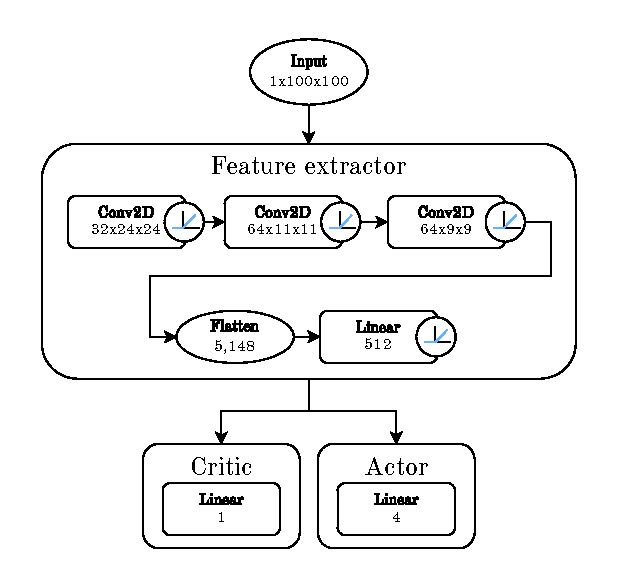
\includegraphics[width=1\linewidth]{diagrams/cnn_arch.pdf}
    \caption{Architecture used by SB3's \texttt{CnnPolicy}.}
    \label{fig:cnn_policy}
\end{figure}

\begin{figure}
    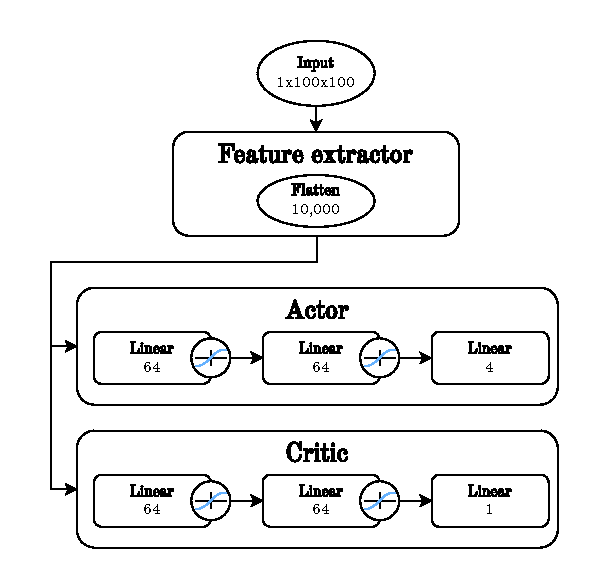
\includegraphics[width=1\linewidth]{diagrams/mlp_arch.pdf}
    \caption{Architecture used by SB3's \texttt{MlpPolicy}.}
    \label{fig:mlp_policy}
\end{figure}

\begin{figure}
    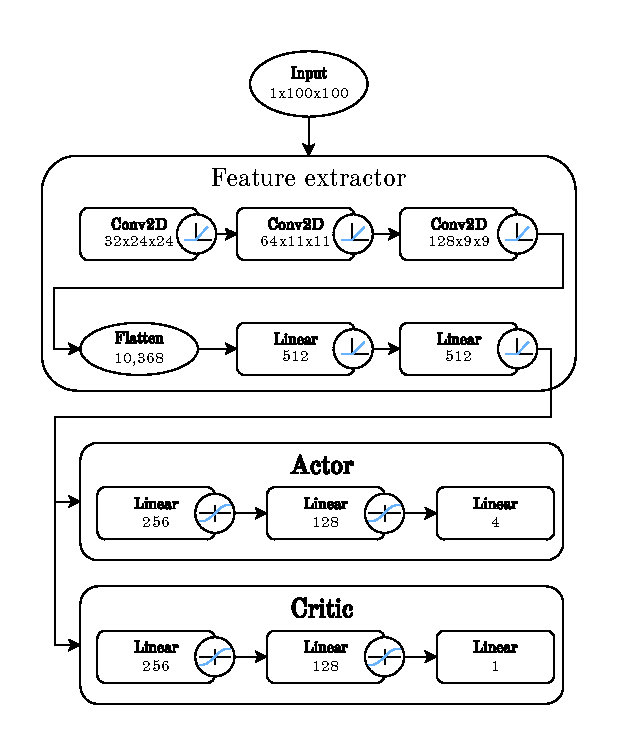
\includegraphics[width=1\linewidth]{diagrams/bigger_net_arch.pdf}
    \caption{Architecture of the network used in Subsection \ref{subsec:arch_change}.}
    \label{fig:bigger_net_policy}
\end{figure}

\begin{figure}
    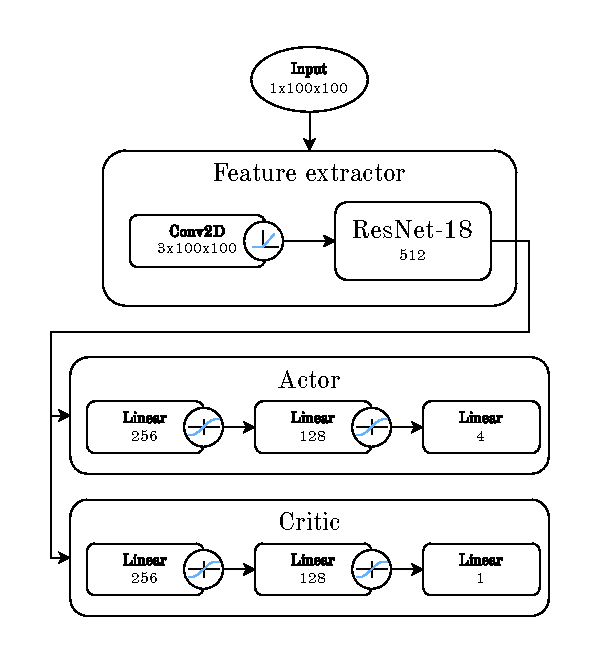
\includegraphics[width=1\linewidth]{diagrams/resnet_arch.pdf}
    \caption{Architecture of the network with a ResNet-18 feature extractor used in Subsection \ref{subsec:resnet}.}
    \label{fig:resnet_arch}
\end{figure}

\end{document}
